\section{Consuntivo e preventivo a finire}
\label{sec:consuntivo}
Sono di seguito indicati i costi sostenuti effettivamente, in relazione alle spese rendicontate, per ogni ruolo.
In corrispondenza di ogni attività del progetto viene redatto un bilancio che può essere:
\begin{itemize}
	\item \textbf{Positivo} se la cifra risultante nel consuntivo risulta inferiore alla cifra preventivata;
	\item \textbf{In pari} se la cifra risultante nel consuntivo è equivalente alla cifra preventivata;	
	\item \textbf{Negativo} se la cifra risultante nel consuntivo risulta superiore alla cifra preventivata.
\end{itemize}
	\subsection{Analisi dei requisiti di massima}
		\subsubsection{Variazioni della pianificazione}
		Durante l'\textit{Analisi dei Requisiti di massima} non sono state necessarie variazioni temporali rispetto a quanto era stato pianificato in origine.
		\subsubsection{Variazione ore e costi}
		Nella seguente tabella è riportata la suddivisione del lavoro effettuata da ogni componente del gruppo
			\begin{table}[H]
			\centering
			\begin{tabular}{|C{4cm}|C{1cm}|C{1cm}|C{1cm}|C{1cm}|C{1cm}|C{1cm}|C{3cm}|}
				\hlineB{3}
				\thead{Nominativo} &\thead{Pm} &\thead{Am} &\thead{An}&\thead{Pt}&\thead{Pr}&\thead{Ve}&\thead{Ore totali}\\
				\hline
				Paolo Eccher        & -  & 3 & 13 & - & - & 6 & 22 \\
				\hline
				Alberto Gallinaro   & -  & - & 16 & - & - & 6 & 22 \\
				\hline
				Giuseppe Merlino    & 10 (-3) & - & 4 (+2) & - & - & 8 (+1) & 22 (-1) \\
				\hline
				Elia Montecchio     & -  & 4 (+1) & 12 & - & - & 8 & 24 (+1) \\
				\hline
				Lisa Parma          & -  & 6 & 12 & - & - & 4 & 22 \\
				\hline
				Francesco Parolini  & 13 & 4 & - & - & - & 6 & 23 \\
				\hline
				Davide Zago         & 5  & 2 & 10 & - & - & 6 & 23 \\
				\hlineB{3}
				\textbf{Ore totali ruolo}  & \textbf{28 (-1)} & \textbf{19 (+1)} & \textbf{65 (+2)} & \textbf{-} & \textbf{-} & \textbf{43} & \textbf{157} \\
				\hlineB{3}
			\end{tabular}
			\caption{Suddivisione del lavoro - \textit{Analisi dei Requisiti di Massima}}	
		\end{table}
		
		
		Nella seguente tabella sono indicate le ore effettive ricoperte per ogni ruolo e la spesa corrispondente durante l'attività di investimento di risorse iniziale per l'approfondimento personale. Queste ore fanno dunque parte delle ore non rendicontate.
		
		\begin{table}[H]
		\centering
		\begin{tabular}{|p{3.8cm}|C{2.6cm}|C{2.9cm}|C{2.7cm}|C{3.3cm}|}
			\hlineB{3}
			
			\thead{Ruolo} &\thead{Ore previste} &\thead{Differenza ore} &\thead{Costo} &\thead{Differenza costo} \\
			\hlineB{3}			
			Project Manager  & 31 & -3 & 930,00\euro & -90,00\euro \\
			\hline
			Amministratore& 18 & +1 & 360,00\euro & +20,00\euro \\
			\hline
			Analista      & 65 & +2 & 1.625,00\euro & +50,00\euro \\
			\hline
			Progettista   & -  & - & 0\euro & 0\euro \\
			\hline
			Programmatore & -  & - & 0\euro & 0\euro \\
			\hline
			Verificatore  & 54 & +1 & 810,00\euro & +15,00\euro \\
			\hlineB{3}
			\textbf{Totale Preventivo} & \textbf{157} & \textbf{-} & \textbf{3.560,00\euro} & \textbf{-}\\
			\hlineB{3}			
			\textbf{Totale Consuntivo} & \textbf{158} & \textbf{+1} & \textbf{3.555,00\euro} & \textbf{-5,00\euro}\\
			
			
			\hlineB{3}
		\end{tabular}
		\caption{Consuntivo - \textit{Analisi dei Requisiti di massima}}
		
		\end{table}
		\subsubsection{Preventivo a finire}
		Al gruppo sono servite un totale di quattro ore aggiuntive. Di queste quattro: una è servita per l'attività di amministrazione, due per quella di analisi e la rimanente ora per la verifica. Inoltre sono risultate sufficienti tre ore in meno di quante preventivate per il ruolo di \textit{Project Manager}.
		Il bilancio finale è un risparmio di \textbf{5,00\euro}. Tuttavia non essendo le ore di questa attività rendicontate questo risparmio non va ad incidere sul valore preventivato che rimane essere \textbf{13,770.00\euro}.


%%%%%%%%%%%%%%%%%%%%%%%%%%%%%%%%%%%%%%%%%%%%%%%%%%%%%%%%
%%%%%%%%%%%%%%%%%%%%%%%%%%%%%%%%%%%%%%%%%%%%%%%%%%%%%%%%
%%%%%%%%%%%%%%%%%%%%%%%%%%%%%%%%%%%%%%%%%%%%%%%%%%%%%%%%
%%%%%%%%%%%%%%%%%%%%%%%%%%%%%%%%%%%%%%%%%%%%%%%%%%%%%%%%


	
	
\subsection{Analisi dei requisiti di dettaglio}
\subsubsection{Variazioni della pianificazione}
Durante l'\textit{Analisi dei Requisiti di dettaglio} sono stati impiegate più ore di quante previste per effettuare la correzione e l'incremento del documento \textit{Analisi dei Requisiti v1.0.0}. Nello stesso tempo sono state necessarie meno ore del previsto per la correzione del documento \textit{Piano di Qualifica v1.0.0}.
\subsubsection{Variazione ore e costi}
Nella seguente tabella è riportata la suddivisione del lavoro effettuata da ogni componente del gruppo

\begin{table}[H]
	\centering
	\begin{tabular}{|C{4cm}|C{1cm}|C{1cm}|C{1cm}|C{1cm}|C{1cm}|C{1cm}|C{3cm}|}
		\hlineB{3}
		\thead{Nominativo} &\thead{Pm} &\thead{Am} &\thead{An}&\thead{Pt}&\thead{Pr}&\thead{Ve}&\thead{Ore totali}\\
		\hlineB{3}
		Paolo Eccher        & - & 3 & 3 & - & - & - & 6 \\
		\hline				
		Alberto Gallinaro   & - & - & 4 & - & - & 2 & 6 \\
		\hline
		Giuseppe Merlino    & - & - & 5 (+1) & - & - & 2 (-1) & 7 \\
		\hline
		Elia Montecchio     & - & - & 3 & - & - & 2 (-1) & 5 (-1) \\
		\hline
		Lisa Parma          & 4 (-2) & - & - & - & - & - & 4 (-2) \\
		\hline
		Francesco Parolini  & 4 & - & 2 & - & - & - & 6 \\
		\hline
		Davide Zago         & - & - & 4 (+1) & - & - & 2 & 6 (+1) \\
		\hlineB{3}
		\textbf{Ore totali ruolo}  & \textbf{8 (-2)} & \textbf{3} & \textbf{21 (+2)} & \textbf{-} & \textbf{-} & \textbf{8 (-2)} & \textbf{40 (-2)} \\
		\hlineB{3}
	\end{tabular}
	\caption{Suddivisione del lavoro - \textit{Analisi dei Requisiti di Dettaglio}}
\end{table}



Nella seguente tabella sono indicate le ore effettive ricoperte per ogni ruolo e la spesa corrispondente durante l'attività di \textit{Analisi dei Requisiti di dettaglio}.
\label{sec:tabellaConsuntivoAdRdD}
\begin{table}[H]
	\centering
	\begin{tabular}{|p{3.8cm}|C{2.6cm}|C{2.9cm}|C{2.7cm}|C{3.3cm}|}
		\hlineB{3}
		
		\thead{Ruolo} &\thead{Ore previste} &\thead{Differenza ore} &\thead{Costo} &\thead{Differenza costo} \\
		\hlineB{3}			
		Project Manager  & 10 & -2 & 300,00\euro & -60,00\euro \\
		\hline
		Amministratore& 3 & - & 60,00\euro & 0\euro \\
		\hline
		Analista      & 19 & +2 & 475,00\euro & +50,00\euro \\
		\hline
		Progettista   & -  & - & 0\euro & 0\euro \\
		\hline
		Programmatore & -  & - & 0\euro & 0\euro \\
		\hline
		Verificatore  & 10 & -2 & 150,00\euro & -30,00\euro \\
		\hlineB{3}
		\textbf{Totale Preventivo} & \textbf{42} & \textbf{-} & \textbf{985,00\euro} & \textbf{-}\\
		\hlineB{3}			
		\textbf{Totale Consuntivo} & \textbf{40} & \textbf{-2} & \textbf{945,00\euro} & \textbf{-40,00\euro}\\
		\hlineB{3}
	\end{tabular}
	\caption{Consuntivo - \textit{Analisi dei Requisiti di dettaglio}}
	
\end{table}
\subsubsection{Preventivo a finire}
Al gruppo complessivamente è servita un ora aggiuntiva. Sono risultate necessarie due ore aggiuntive per il ruolo di \textit{Analista}, in quanto gli incrementi e le correzioni all'\textit{Analisi dei Requisiti} sono stati più ingenti del previsto. Allo stesso tempo si sono potute risparmiare 2 ore previste per il ruolo di \textit{Verificatore}, poichè il \textit{Piano di Qualifica} ha necessitato meno attenzioni di quanto preventivato e 2 ore per il ruolo \textit{Project Manager}. Il bilancio finale è un risparmio di \textbf{40,00\euro} rispetto a quanto inizialmente preventivato. Il preventivo rimane invariato a \textbf{13.770,00\euro}, poichè i \textbf{40\euro}  potrebbero servire come margine per aggiungere ore di lavoro nel futuro.


%%%%%%%%%%%%%%%%%%%%%%%%%%%%%%%%%%%%%%%%%%%%%%%%%%%%%%%%
%%%%%%%%%%%%%%%%%%%%%%%%%%%%%%%%%%%%%%%%%%%%%%%%%%%%%%%%
%%%%%%%%%%%%%%%%%%%%%%%%%%%%%%%%%%%%%%%%%%%%%%%%%%%%%%%%
%%%%%%%%%%%%%%%%%%%%%%%%%%%%%%%%%%%%%%%%%%%%%%%%%%%%%%%%




\subsection{Progettazione architetturale}
\subsubsection{Variazioni della pianificazione}
Durante la \textit{Progettazione architetturale} è stata variata sensibilmente la pianificazione del lavoro. In particolare si sono rese necessarie parecchie ore del ruolo \textit{Programmatore} per preparare il \textit{Proof of Concept}. Si sono tuttavia diminuite le ore del \textit{Progettista}.

\subsubsection{Variazione ore e costi}
Nella seguente tabella sono indicate le ore effettive ricoperte per ogni ruolo e la spesa corrispondente durante l'attività di \textit{Progettazione architetturale}.

Nella seguente tabella è riportata la suddivisione del lavoro effettuata da ogni componente del gruppo
\begin{table}[H]
	\centering
	\begin{tabular}{|C{4cm}|C{1cm}|C{1cm}|C{1cm}|C{1cm}|C{1cm}|C{1cm}|C{2.5cm}|}
		\hlineB{3}
		\thead{Nominativo} &\thead{Pm} &\thead{Am} &\thead{An}&\thead{Pt}&\thead{Pr}&\thead{Ve}&\thead{Ore totali}\\
		\hlineB{3}
		Paolo Eccher      & 5 (-1) & - & - & 4 (-14) & 12 (+12) & 6 & 27 (+1) \\
		\hline
		Alberto Gallinaro & - & 3 & - & 8 (-9) & 10 (+10) & 5 & 26 (+1) \\
		\hline
		Giuseppe Merlino  & - & - & - & 10 (-5) & 6 (+6) & 10 & 26 (+1) \\
		\hline
		Elia Montecchio   & 3 & - & - & 10 (-2) & - & 10 & 23 (-2) \\
		\hline
		Lisa Parma        & 2 (+1) & - & - & 16 & - & 9 & 27 (+1) \\
		\hline
		Francesco Parolini& - & 5 & - & 8 (-2) & 8 (+8) & 4 (-6) & 25 \\
		\hline
		Davide Zago       & 3 (+3) & - & - & 7 (-11) & - & 15 (+8) & 25 \\
		\hline
		\textbf{Ore totali ruolo}  & \textbf{13 (+3)} & \textbf{8} & \textbf{0} & \textbf{63 (-39)} & \textbf{36 (+36)} & \textbf{59 (+2)} & \textbf{179 (+2)} \\
		\hlineB{3}
	\end{tabular}
	\caption{Suddivisione del lavoro - \textit{Progettazione Architetturale}}
\end{table}

Nella seguente tabella sono indicate le ore effettive ricoperte per ogni ruolo e la spesa corrispondente durante l'attività di \textit{Progettazione Architetturale}.

\label{sec:tabellaConsuntivoPA}
\begin{table}[H]
	\centering
	\begin{tabular}{|p{3.8cm}|C{2.6cm}|C{2.9cm}|C{2.7cm}|C{3.3cm}|}
		\hlineB{3}
		
		\thead{Ruolo} &\thead{Ore previste} &\thead{Differenza ore} &\thead{Costo} &\thead{Differenza costo} \\
		\hlineB{3}			
		Project Manager  & 10 & +3 & 300,00\euro & +90,00\euro \\
		\hline
		Amministratore& 8 & - & 160,00\euro & 0\euro \\
		\hline
		Analista      & - & - & 0,00\euro & 0\euro \\
		\hline
		Progettista   & 102  & -39 & 1.452,00\euro & -856,00\euro \\
		\hline
		Programmatore & 0  & +36 & 540,00\euro & +540,00\euro \\
		\hline
		Verificatore  & 57 & +2 & 855,00\euro & +30,00\euro \\
		\hlineB{3}
		\textbf{Totale Preventivo} & \textbf{177} & \textbf{-} & \textbf{3.427,00\euro} & \textbf{-}\\
		\hlineB{3}			
		\textbf{Totale Consuntivo} & \textbf{179} & \textbf{+2} & \textbf{3.361,00\euro} & \textbf{-198,00\euro}\\
		\hlineB{3}
	\end{tabular}
	\caption{Consuntivo - \textit{Progettazione architetturale}}



\end{table}

\subsubsection{Preventivo a finire}
Il cambiamento nella pianificazione attuato per riuscire a produrre il \textit{Proof of Concept} ha delle ricadute sull'organizzazione futura del lavoro. In particolare, l'esperienza che verrà maturata applicando le tecnologie dominio del prodotto ci permetterà di velocizzare il compito del \textit{Programmatore} durante il proseguo del lavoro. Allo stesso modo, le ore di lavoro del \textit{Progettista}, che sono state dirottate verso il \textit{Programmatore} per riuscire a sviluppare il \textit{Proof of Concept}. Il bilancio di questa attività è un risparmio di \textbf{198,00\euro} a causa della diminuzione di ore per il \textit{Progettista}. Tuttavia una parte di tali ore verrà recuperata nel proseguo del progetto, per garantire lo sviluppo di un prodotto con un'adeguata archittettura. Riteniamo dunque ragionevole mantenere il preventivo stabile a \textbf{13.770,00\euro} per poter gestire eventuali fluttuazioni future.


%%%%%%%%%%%%%%%%%%%%%%%%%%%%%%%%%%%%%%%%%%%%%%%%%%%%%%%%
%%%%%%%%%%%%%%%%%%%%%%%%%%%%%%%%%%%%%%%%%%%%%%%%%%%%%%%%
%%%%%%%%%%%%%%%%%%%%%%%%%%%%%%%%%%%%%%%%%%%%%%%%%%%%%%%%
%%%%%%%%%%%%%%%%%%%%%%%%%%%%%%%%%%%%%%%%%%%%%%%%%%%%%%%%



\subsection{Progettazione di Dettaglio}
\label{sec:ConsuntivoProgettazioneDettaglio}
\subsubsection{Variazioni della pianificazione}
Durante la \textit{Progettazione di Dettaglio} la pianificazione non ha subito variazioni significative.

\subsubsection{Variazione ore e costi}
Nella seguente tabella sono indicate le ore effettive ricoperte per ogni ruolo e la spesa corrispondente durante l'attività di \textit{Progettazione di Dettaglio}.

Nella seguente tabella è riportata la suddivisione del lavoro effettuata da ogni componente del gruppo


\begin{table}[H]
	\centering
	\begin{tabular}{|C{4.5cm}|C{1cm}|C{1cm}|C{1cm}|C{1cm}|C{1cm}|C{1cm}|C{3cm}|}
		\hlineB{3}
		\thead{Nominativo} &\thead{Pm} &\thead{Am} &\thead{An}&\thead{Pt}&\thead{Pr}&\thead{Ve}&\thead{Ore totali}\\
		\hlineB{3}
		Paolo Eccher      & - & - & - & 18 (-5) & - & 5 (+5) & 23 \\
		\hline
		Alberto Gallinaro & 4 (-2) & - & - & 16 & - & 4 (+2) & 24 \\
		\hline
		Giuseppe Merlino  & - & - & - & 2 & - & 19 (-1) & 21 (-1)\\
		\hline
		Elia Montecchio   & 2 & - & - & 5 (+5) & - & 17 (-5) & 24 \\
		\hline 
		Lisa Parma        & - & 3 & - & 20 & - & 0 & 23 \\
		\hline
		Francesco Parolini& - & - & - & 17 & - & 6 & 23 \\
		\hline
		Davide Zago       & - & 4 & - & 13 (-1) & - & 5 & 22 (-1) \\
		\hline
		\textbf{Ore totali ruolo}  & \textbf{6 (-2)} & \textbf{7} & \textbf{-} & \textbf{91 (-1)} & \textbf{-} & \textbf{56 (+1)} & \textbf{160 (-2)} \\
		\hlineB{3}
	\end{tabular}
	\caption{Nuova suddivisione del lavoro - \textit{Progettazione di dettaglio}}
\end{table}



Nella seguente tabella sono indicate le ore effettive ricoperte per ogni ruolo e la spesa corrispondente durante l'attività di \textit{Progettazione di Dettaglio}.

\begin{table}[H]
	\centering
	\begin{tabular}{|p{3.8cm}|C{2.6cm}|C{2.9cm}|C{2.7cm}|C{3.3cm}|}
		\hlineB{3}
		
		\thead{Ruolo} &\thead{Ore previste} &\thead{Differenza ore} &\thead{Costo} &\thead{Differenza costo} \\
		\hlineB{3}			
		Project Manager & 8 & -2 & 180,00\euro & -60,00\euro  \\
		\hline
		Amministratore& 7 & - & 140,00\euro & 0\euro \\
		\hline
		Analista & - & - & 0\euro & 0\euro \\
		\hline
		Progettista & 91 & -1 & 2.002,00\euro & -22,00\euro \\
		\hline
		Programmatore & - & - & 0\euro & 0\euro \\
		\hline
		Verificatore & 55 & +1 & 840,00\euro & +15,00\euro \\
		\hlineB{3}
		\textbf{Totale Preventivo} & \textbf{162} & \textbf{-} & \textbf{3.229,00\euro} & \textbf{-}\\
		\hlineB{3}			
		\textbf{Totale Consuntivo} & \textbf{160} & \textbf{-2} & \textbf{3.162,00\euro} & \textbf{-67,00\euro}\\
		\hlineB{3}
		
		
	\end{tabular}
	\caption{Costi per ruolo - \textit{Progettazione di dettaglio}}
\end{table}



\subsubsection{Preventivo a finire}
Il lavoro non ha subito grosse variazioni se non un aggiunta di un ora del ruolo \textit{Verificatore} ed il risparmio di un ora di \textit{Progettista} e due di \textit{Project Manager}. Il bilancio di questa è dunque in positivo grazie ad un risparmio di \textbf{67,00\euro}. Riteniamo tuttavia opportuno mantenere il preventivo stabile a \textbf{13.770,00\euro} per poter gestire future fluttuazioni.


%%%%%%%%%%%%%%%%%%%%%%%%%%%%%%%%%%%%%%%%%%%%%%%%%%%%%%%%
%%%%%%%%%%%%%%%%%%%%%%%%%%%%%%%%%%%%%%%%%%%%%%%%%%%%%%%%
%%%%%%%%%%%%%%%%%%%%%%%%%%%%%%%%%%%%%%%%%%%%%%%%%%%%%%%%
%%%%%%%%%%%%%%%%%%%%%%%%%%%%%%%%%%%%%%%%%%%%%%%%%%%%%%%%s


\subsection{Codifica}
\label{sec:ConsuntivoCodifica}
\subsubsection{Variazioni della pianificazione}
Durante la \textit{Codifica} è stata variata sensibilmente la pianificazione del lavoro. In particolare si sono rese necessarie parecchie ore del ruolo \textit{Progettista} per preparare la \textit{Product Baseline}. Si sono tuttavia diminuite le ore del \textit{Programmatore}.

\subsubsection{Variazione ore e costi}
Nella seguente tabella sono indicate le ore effettive ricoperte per ogni ruolo e la spesa corrispondente durante l'attività di \textit{Progettazione architetturale}.

Nella seguente tabella è riportata la suddivisione del lavoro effettuata da ogni componente del gruppo
\begin{table}[H]
	\centering
	\begin{tabular}{|C{4cm}|C{1cm}|C{1cm}|C{1cm}|C{1cm}|C{1cm}|C{1cm}|C{2.5cm}|}
		\hlineB{3}
		\thead{Nominativo} &\thead{Pm} &\thead{Am} &\thead{An}&\thead{Pt}&\thead{Pr}&\thead{Ve}&\thead{Ore totali}\\
		\hlineB{3}
		Paolo Eccher      & - & - & - & 15 (+4) & 5 (-5) & 13 & 32 (-1) \\
		\hline
		Alberto Gallinaro & 4 (-1) & - & - & 14 (+4) & 14 (-4) & - & 32 (-1) \\
		\hline
		Giuseppe Merlino  & - & 6 & - & - & 28 & - & 34 \\
		\hline
		Elia Montecchio   & - & - & - & 8 (+8) & 6 (-7) & 20 & 34 (+1) \\
		\hline
		Lisa Parma        & - & - & - & - & 13 & 20 & 33 \\
		\hline
		Francesco Parolini& - & - & - & 10 (+3) & 15 (-3) & 9 & 34 \\
		\hline
		Davide Zago       & 5 (-1) & - & - & 10 (+10) & 10 (-10) & 8 & 33 (-1) \\
		\hline
		\textbf{Ore totali ruolo}  & \textbf{9 (-2)} & \textbf{6} & \textbf{-} & \textbf{56 (+29)} & \textbf{91 (-29)} & \textbf{70} & \textbf{232(-2)} \\
		\hlineB{3}
	\end{tabular}
	\caption{Suddivisione del lavoro - \textit{Codifica}}
\end{table}

Nella seguente tabella sono indicate le ore effettive ricoperte per ogni ruolo e la spesa corrispondente durante l'attività di \textit{Codifica}.

\label{sec:tabellaConsuntivoPA}
\begin{table}[H]
	\centering
	\begin{tabular}{|p{3.8cm}|C{2.6cm}|C{2.9cm}|C{2.7cm}|C{3.3cm}|}
		\hlineB{3}
		
		\thead{Ruolo} &\thead{Ore previste} &\thead{Differenza ore} &\thead{Costo} &\thead{Differenza costo} \\
		\hlineB{3}			
		Project Manager & 11 & -2 & 270,00\euro & -60,00\euro \\
		\hline
		Amministratore & 6 & - & 120,00\euro & 0\euro \\
		\hline
		Analista      & - & - & 0,00\euro & 0\euro \\
		\hline
		Progettista   & 27  & +29 & 1.232,00\euro & +638,00\euro \\
		\hline
		Programmatore & 120 & -29 & 1.365,00\euro & -435,00\euro \\
		\hline
		Verificatore  & 70 & - & 1050,00\euro & 0\euro \\
		\hlineB{3}
		\textbf{Totale Preventivo} & \textbf{234} & \textbf{-} & \textbf{3.894,00\euro} & \textbf{-}\\
		\hlineB{3}			
		\textbf{Totale Consuntivo} & \textbf{232} & \textbf{-2} & \textbf{4.037,00\euro} & \textbf{+143,00\euro}\\
		\hlineB{3}
	\end{tabular}
	\caption{Consuntivo - \textit{Codifica}}
	
\end{table}

\subsubsection{Preventivo a finire}
In questa attività sono state aggiunte ben 29 ore del ruolo \textit{Progettista} per la redazione della \textit{Product Baseline}. Sono state allo stesso tempo risparmiate 29 ore del ruolo \textit{Programmatore} poichè si è riusciti a recuperare buona parte del lavoro preparato in precedenza sotto forma di \textit{Proof of Concept}. A causa del maggior costo del ruolo \textit{Progettista} rispetto al \textit{Programmatore} il bilancio di questa attività è in \textbf{negativo di 143,00\euro}. Tale saldo negativo tuttavia non inficia la validità della nostra offerta dato che nelle attività precedenti abbiamo accumulato un risparmio di \textbf{305,00\euro}. 
Questo aumento viene però ammortizzato dal risparmio conseguito nelle attività precedenti che ammonta a \textbf{305,00\euro}. Riteniamo dunque saggio, considerato anche che l'aver accumulato risparmio in precedenza ci è stato utile, di mantenere il bilancio stabile a \textbf{13.770,00\euro}.



%%%%%%%%%%%%%%%%%%%%%%%%%%%%%%%%%%%%%%%%%%%%%%%%%%%%%%%%
%%%%%%%%%%%%%%%%%%%%%%%%%%%%%%%%%%%%%%%%%%%%%%%%%%%%%%%%
%%%%%%%%%%%%%%%%%%%%%%%%%%%%%%%%%%%%%%%%%%%%%%%%%%%%%%%%
%%%%%%%%%%%%%%%%%%%%%%%%%%%%%%%%%%%%%%%%%%%%%%%%%%%%%%%%



\subsection{Settimana dal 04/23 al 04/29 }
\label{sec:Consuntivo1Sett}
\subsubsection{Variazioni della pianificazione}

Come deciso a verbale \textit{VI\_2018-04-22} il gruppo ha deciso di darsi una nuova pianificazione, con due obiettivi principali:
\begin{itemize}
	\item porre più attenzione sulla validazione prodotto da realizzare;
	\item implementare pienamente il modello di sviluppo incrementale.
\end{itemize}

A seguito di tale cambiamento il gruppo ha deciso di abbandonare la suddivisione in periodi, andando piuttosto a scansionare il lavoro rimanente settimana per settimana, con riscontri organizzativi e di qualità calcolati alla fine della settimana considerata. Inoltre il lavoro non è più stato  incentrato sul raggiungimento di obiettivi scanditi dalle date delle revisioni, ma è stato diviso per rispettare gli impegni del gruppo e permettere di lavorare in maniera efficace al prodotto. Di seguito i diagrammi di Gantt della nuova pianificazione adottata, divisi tra documentazione e prodotto semplicemente per una questione di maggiore leggibilità.


\subsubsection{Variazione ore e costi}
Nella seguente tabella è riportata la suddivisione del lavoro effettuata da ogni componente del gruppo
\begin{table}[H]
	\centering
	\begin{tabular}{|C{4cm}|C{1cm}|C{1cm}|C{1cm}|C{1cm}|C{1cm}|C{1cm}|C{2.5cm}|}
		\hlineB{3}
		\thead{Nominativo} &\thead{Pm} &\thead{Am} &\thead{An}&\thead{Pt}&\thead{Pr}&\thead{Ve}&\thead{Ore totali}\\
		\hlineB{3}
		Paolo Eccher      & - & - & - & 2 & - & 11 & 13 \\
		\hline
		Alberto Gallinaro & - & 2 & - & - & - & 7 & 9 \\
		\hline
		Giuseppe Merlino  & - & - & - & 3 & - & 5 & 8 \\
		\hline
		Elia Montecchio   & - & - & - & 3 (-1) & 4 (+4) & 6 & 13 (+3) \\
		\hline
		Lisa Parma        & - & - & 2 (+2) & 4 (-1) & - & - & 9 (+1) \\
		\hline
		Francesco Parolini& 2 & - & - & - & 2 (+2) & 6 (-2) & 10 \\
		\hline
		Davide Zago       & 1 (-1) & - & - & - & - & 6 & 7 (-1) \\
		\hline
		\textbf{Ore totali ruolo}  & \textbf{3 (-1)} & \textbf{2} & \textbf{2 (+2)} & \textbf{12 (-2)} & \textbf{6 (+6)} & \textbf{44 (-2)} & \textbf{69 (+3)} \\
		\hlineB{3}
	\end{tabular}
	\caption{Suddivisione del lavoro - \textit{Settimana dal 04/23 al 04/29}}
\end{table}

Nella seguente tabella sono indicate le ore effettive ricoperte per ogni ruolo e la spesa corrispondente durante la \textit{settimana dal 04/23 al 04/29}.

\label{sec:tabellaConsuntivo1Sett}
\begin{table}[H]
	\centering
	\begin{tabular}{|p{3.8cm}|C{2.6cm}|C{2.9cm}|C{2.7cm}|C{3.3cm}|}
		\hlineB{3}
		
		\thead{Ruolo} &\thead{Ore previste} &\thead{Differenza ore} &\thead{Costo} &\thead{Differenza costo} \\
		\hlineB{3}			
		Project Manager & 3 & -1 & 90,00\euro & -30,00\euro \\
		\hline
		Amministratore & 2 & - & 40,00\euro & 0\euro \\
		\hline
		Analista      & 2 & +2 & 50,00\euro & +50,00\euro \\
		\hline
		Progettista   & 12 & -2 & 264,00\euro & +44,00\euro \\
		\hline
		Programmatore & 6 & +6 & 90,00\euro & +90,00\euro \\
		\hline
		Verificatore  & 44 & -2 & 660,00\euro & -30,00\euro \\
		\hlineB{3}
		\textbf{Totale Preventivo} & \textbf{66} & \textbf{-} & \textbf{1.194,00\euro} & \textbf{-}\\
		\hlineB{3}			
		\textbf{Totale Consuntivo} & \textbf{69} & \textbf{+3} & \textbf{1.158,00\euro} & \textbf{+36,00\euro}\\
		\hlineB{3}
	\end{tabular}
	\caption{Consuntivo - \textit{Settimana dal 04/23 al 04/29}}
	
\end{table}

\subsubsection{Preventivo a finire}
Nel corso di questa settimana si sono rese necessarie 2 ore del ruolo \textit{Analista} per poter porre alcune modifiche concordate con il proponente al documento \textit{Analisi dei Requisiti}. Inoltre sono state necessarie 6 ore di \textit{Programmatore} per riuscire a soddisfare degli ultimi requisiti richiesti dal proponente. Al contempo sono risultate essere sueprflue 2 ore del ruolo \textit{Progettista} , 2 ore di \textit{Verificatore} e 1 di {Project Manager}. Il bilancio di questa settimana è in negativo di \textbf{36,00\euro}. Questa mancanza viene però colmata dal risparmio accumulato in precedenza. Il bilancio rimane dunque stabile a \textbf{13.770,00\euro}.  





%%%%%%%%%%%%%%%%%%%%%%%%%%%%%%%%%%%%%%%%%%%%%%%%%%%%%%%%
%%%%%%%%%%%%%%%%%%%%%%%%%%%%%%%%%%%%%%%%%%%%%%%%%%%%%%%%
%%%%%%%%%%%%%%%%%%%%%%%%%%%%%%%%%%%%%%%%%%%%%%%%%%%%%%%%
%%%%%%%%%%%%%%%%%%%%%%%%%%%%%%%%%%%%%%%%%%%%%%%%%%%%%%%%



\subsection{Settimana dal 04/30 al 05/05 }
\label{sec:Consuntivo2Sett}
\subsubsection{Variazioni della pianificazione}
Durante la \textit{Settimana dal 04/30 al 05/05 }, non è stata variata sensibilmente la pianificazione del lavoro.
\subsubsection{Variazione ore e costi}
Nella seguente tabella sono indicate le ore effettive ricoperte per ogni ruolo e la spesa corrispondente durante la \textit{settimana dal 04/30 al 05/05 }.

Nella seguente tabella è riportata la suddivisione del lavoro effettuata da ogni componente del gruppo
\begin{table}[H]
	\centering
	\begin{tabular}{|C{4cm}|C{1cm}|C{1cm}|C{1cm}|C{1cm}|C{1cm}|C{1cm}|C{2.5cm}|}
		\hlineB{3}
		\thead{Nominativo} &\thead{Pm} &\thead{Am} &\thead{An}&\thead{Pt}&\thead{Pr}&\thead{Ve}&\thead{Ore totali}\\
		\hlineB{3}
		Paolo Eccher      & - & - & - & - & - & 4 & 4 \\
		\hline
		Alberto Gallinaro & - & 1 & - & - & - & 7 & 8 \\
		\hline
		Giuseppe Merlino  & - & - & - & 2 & - & 7 & 9 \\
		\hline
		Elia Montecchio   & - & - & - & 2 (-1) & - & 4 & 6 (-1) \\
		\hline
		Lisa Parma        & - & - & - & 4 (-1) & - & 5 (+1) & 9 \\
		\hline
		Francesco Parolini& - & - & - & - & - & 7 & 7 \\
		\hline
		Davide Zago       & 3 (-1) & - & - & 2 (+2) & - & 7 (+1) & 12 (+2) \\
		\hline
		\textbf{Ore totali ruolo}  & \textbf{3 (-1)} & \textbf{1} & \textbf{-} & \textbf{10} & \textbf{-} & \textbf{41 (+2)} & \textbf{55 (+1)} \\
		\hlineB{3}
	\end{tabular}
	\caption{Suddivisione del lavoro - \textit{Settimana dal 04/30 al 05/05 }}
\end{table}

Nella seguente tabella sono indicate le ore effettive ricoperte per ogni ruolo e la spesa corrispondente durante la \textit{settimana dal 04/30 al 05/05 }.

\label{sec:tabellaConsuntivo2Sett}
\begin{table}[H]
	\centering
	\begin{tabular}{|p{3.8cm}|C{2.6cm}|C{2.9cm}|C{2.7cm}|C{3.3cm}|}
		\hlineB{3}
		
		\thead{Ruolo} &\thead{Ore previste} &\thead{Differenza ore} &\thead{Costo} &\thead{Differenza costo} \\
		\hlineB{3}			
		Project Manager & 3 & -1 & 90,00\euro & -30,00\euro \\
		\hline
		Amministratore & 1 & - & 20,00\euro & 0\euro \\
		\hline
		Analista      & - & - & 0\euro & 0\euro \\
		\hline
		Progettista   & 10 & - & 220,00\euro & 0\euro \\
		\hline
		Programmatore & - & - & 0\euro & 0\euro \\
		\hline
		Verificatore  & 41 & +2 & 615,00\euro & +30,00\euro \\
		\hlineB{3}
		\textbf{Totale Preventivo} & \textbf{54} & \textbf{-} & \textbf{945,00\euro} & \textbf{-}\\
		\hlineB{3}			
		\textbf{Totale Consuntivo} & \textbf{55} & \textbf{+1} & \textbf{945,00\euro} & \textbf{0\euro}\\
		\hlineB{3}
	\end{tabular}
	\caption{Consuntivo - \textit{Settimana dal 04/30 al 05/05 }}
	
\end{table}

\subsubsection{Preventivo a finire}
Durante la  \textit{settimana dal 04/30 al 05/05} si sono rese necessarie 2 ore in più di quelle preventivate per il ruolo \textit{Verificatore} per accertarsi di consegnare del materiale adeguato. Ne è stata necessaria una in meno per il ruolo \textit{Project Manager}. Il bilancio in questa settimana conclusiva è \textbf{in pari}.


%%%%%%%%%%%%%%%%%%%%%%%%%%%%%%%%%%%%%%%%%%%%%%%%%%%%%%%%
%%%%%%%%%%%%%%%%%%%%%%%%%%%%%%%%%%%%%%%%%%%%%%%%%%%%%%%%
%%%%%%%%%%%%%%%%%%%%%%%%%%%%%%%%%%%%%%%%%%%%%%%%%%%%%%%%
%%%%%%%%%%%%%%%%%%%%%%%%%%%%%%%%%%%%%%%%%%%%%%%%%%%%%%%%



\subsection{Consuntivo Finale}
\label{sec:ConsuntivoFinale}
%
%\subsubsection{Suddivisione del lavoro - Ore totale d'investimento}
%Le ore rendicontate totali sono riassunte nella seguente tabella:
%
%\begin{table}[H]
%	\centering
%	\begin{tabular}{|C{4cm}|C{1cm}|C{1cm}|C{1cm}|C{1cm}|C{1cm}|C{1cm}|C{2.5cm}|}
%		\hlineB{3}
%		\thead{Nominativo} &\thead{Pm} &\thead{Am} &\thead{An}&\thead{Pt}&\thead{Pr}&\thead{Ve}&\thead{Ore totali}\\
%		\hlineB{3}
%		Paolo Eccher      & 5 & 6 & 16 & 38 & 17 & 45 & 127 \\
%		\hline
%		Alberto Gallinaro & 8 & 6 & 20 & 38 & 24 & 31 & 127 \\
%		\hline
%		Giuseppe Merlino  & 10 & 6 & 9 & 17 & 34 & 50 & 126 \\
%		\hline
%		Elia Montecchio   & 5 & 4 & 15 & 28 & 10 & 67 & 129 \\
%		\hline
%		Lisa Parma        & 6 & 9 & 14 & 44 & 13 & 41 & 127 \\
%		\hline
%		Francesco Parolini& 19 & 9 & 2 & 35 & 25 & 38 & 128 \\
%		\hline
%		Davide Zago       & 17 & 6 & 14 & 32 & 10 & 49 & 128 \\
%		\hline
%		\textbf{Ore totali ruolo}  & \textbf{70} & \textbf{46} & \textbf{90} & \textbf{232} & \textbf{133} & \textbf{321} & \textbf{892} \\
%		\hlineB{3}
%		\textbf{Costo totale}  & \textbf{2100\euro} & \textbf{920\euro} & \textbf{2250\euro} & \textbf{5104\euro} & \textbf{1995\euro} & \textbf{4815\euro} & \textbf{17.184\euro} \\
%		\hlineB{3}
%	\end{tabular}
%	\caption{Riepilogo - ore d'investimento totale}
%\end{table}
%
%Tali dati sono riassunti graficamente nei seguenti grafici:
%
%\textcolor{red}{finale totale barre}
%
%\textcolor{red}{finale totale torta}
%


%%%%%%%%%%%%%%%%%%%%%%%%%%%%%%%%%%%%%%%%%%%%%%%%%%%%%%%%
%%%%%%%%%%%%%%%%%%%%%%%%%%%%%%%%%%%%%%%%%%%%%%%%%%%%%%%%
%%%%%%%%%%%%%%%%%%%%%%%%%%%%%%%%%%%%%%%%%%%%%%%%%%%%%%%%
%%%%%%%%%%%%%%%%%%%%%%%%%%%%%%%%%%%%%%%%%%%%%%%%%%%%%%%%



\subsubsection{Suddivisione del lavoro - Ore rendicontate}
Le ore rendicontate totali sono riassunte nella seguente tabella:

\begin{table}[H]
	\centering
	\begin{tabular}{|C{4cm}|C{1cm}|C{1cm}|C{1cm}|C{1cm}|C{1cm}|C{1cm}|C{2.5cm}|}
		\hlineB{3}
		\thead{Nominativo} &\thead{Pm} &\thead{Am} &\thead{An}&\thead{Pt}&\thead{Pr}&\thead{Ve}&\thead{Ore totali}\\
		\hlineB{3}
		Paolo Eccher      & 5 (-1) & 3 & 3 & 38 (-11) & 17 (+7) & 39 (+5) & 105 \\
		\hline
		Alberto Gallinaro & 8 (-3) & 6 & 4 & 38 (-5) & 24 (+6) & 25 (+2) & 105 \\
		\hline
		Giuseppe Merlino  & - & 6 & 5 (+1) & 17 (-5) & 34 (+6) & 43 (-2) & 105 \\
		\hline
		Elia Montecchio   & 5 & - & 3 & 28 (+9) & 10 (-3) & 59 (-6) & 105 \\
		\hline
		Lisa Parma        & 6 (-1) & 3 & 2 (+2) & 44 (-2) & 13 & 37 (+1) & 105 \\
		\hline
		Francesco Parolini& 6 & 5 & 2 & 35 (+1) & 25 (+7) & 32 (-8) & 105 \\
		\hline
		Davide Zago       & 12 & 4 & 4 (+1) & 32 & 10 (-10) & 43 (+9) & 105 \\
		\hline
		\textbf{Ore totali ruolo}  & \textbf{42 (-5)} & \textbf{27} & \textbf{23 (+4)} & \textbf{232 (-13)} & \textbf{133 (+13)} & \textbf{278 (+1)} & \textbf{735} \\
		\hlineB{3}
		\textbf{Costo totale}  & \textbf{1260\euro} & \textbf{540\euro} & \textbf{575\euro} & \textbf{5104\euro} & \textbf{1995\euro} & \textbf{4170\euro} & \textbf{13.644\euro} \\
		\hlineB{3}
	\end{tabular}
	\caption{Consuntivo finale - ore di lavoro rendicontate}
\end{table}

Tali dati sono riassunti graficamente nei seguenti grafici:


\begin{figure}[H] 
	\centering 
	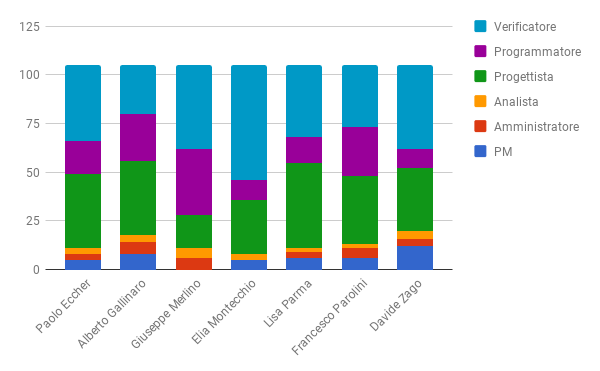
\includegraphics[width=0.9\textwidth]{images/BarreFinaleRendicontate.png} 
	\caption{Diagramma a barre con ripartizione delle ore finale.}
	\label{BarreFinaleRendicontate}
\end{figure}

\begin{figure}[H] 
	\centering 
	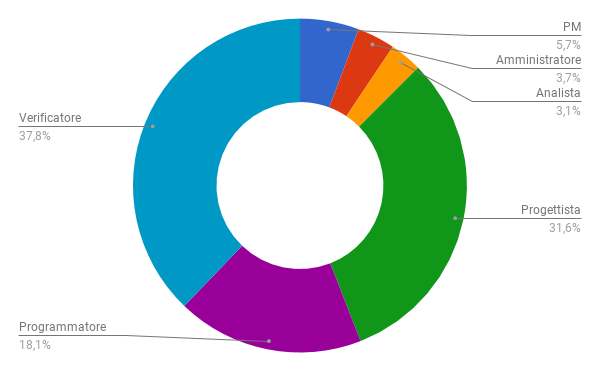
\includegraphics[width=0.9\textwidth]{images/CircolareFinaleRendicontate.png} 
	\caption{Diagramma circolare con ripartizione delle ore finale.}
	\label{CircolareFinaleRendicontate}
\end{figure}

\paragraph{Costi totali} \Spazio
L’impegno in termini di ore rendicontate si attesta a 105 ore a persona, per un totale di 735 ore rendicontate.
Il costo totale a carico del proponente è di \textbf{13.644,00\euro}, con un risparmio di \textbf{126\euro} rispetto a quanto inizialmente preventivato,
